% Three-page discussion brief for supervisors.
% Build from this directory with:
%   tectonic --keep-logs --keep-intermediates --reruns 1 overview.tex
\documentclass[10pt,a4paper]{article}

\usepackage[margin=1.75cm]{geometry}
\usepackage[T1]{fontenc}
\usepackage{lmodern}
\usepackage{microtype}
\usepackage{booktabs}
\usepackage{tabularx}
\usepackage{array}
\usepackage{xcolor}
\usepackage{enumitem}
\usepackage{tikz}
\usetikzlibrary{arrows.meta, positioning}
\usepackage[numbers,sort&compress]{natbib}
\usepackage[colorlinks=true, linkcolor=accent, urlcolor=accent,
            citecolor=accent]{hyperref}

\definecolor{accent}{RGB}{128,0,32}
\definecolor{hbmcol}{RGB}{213,125,28}
\definecolor{neutralcol}{RGB}{235,238,242}
\definecolor{green}{RGB}{48,115,72}
\newcolumntype{Y}{>{\raggedright\arraybackslash}X}
\newcolumntype{P}[1]{>{\raggedright\arraybackslash}p{#1}}
\setlist[itemize]{leftmargin=*, itemsep=1.5pt, topsep=3pt}
\setlist[enumerate]{leftmargin=*, itemsep=1.5pt, topsep=3pt}
\setlength{\parindent}{0pt}
\setlength{\parskip}{3.5pt}
\setlength{\emergencystretch}{2em}
\pagestyle{plain}
\raggedbottom

\newcommand{\researchq}[1]{\textbf{RQ#1}}
\newcommand{\heading}[1]{%
  \vspace{4pt}{\large\bfseries\color{accent}#1}\par
  \vspace{1pt}\hrule height 0.35pt\vspace{4pt}}

\begin{document}

{\LARGE\bfseries Quantized LLM Inference on Xeon Max HBM\par}
\vspace{3pt}
{\large Evidence, proposed thesis gap, and decisions for the first
experimental phase\par}
\vspace{5pt}
Lucian Crainic \hfill Supervisor discussion brief, 26 July 2026

\heading{Purpose}

The proposed thesis studies when on-package HBM changes CPU-only LLM
inference on the CRESCO8 Xeon Max~9480 partition.  The immediate aim is
not to claim general CPU superiority or to redesign an inference
runtime.  It is to isolate memory tier on the same socket, explain the
result through phase, live-set size and locality, and use that evidence
to decide whether finer software placement is worth implementing.

\heading{What the supplied literature establishes}

\begin{table}[h]
\centering
\footnotesize
\begin{tabularx}{\textwidth}{@{}P{2.35cm}YY@{}}
\toprule
\textbf{Work} & \textbf{Achievement} & \textbf{Limit for this thesis} \\
\midrule
Na et al.\ \cite{na2024llmcpu}
& Shows that Xeon Max can be competitive for BF16 inference and that
  memory mode and naive two-socket execution matter.
& Changes hardware and software factors together; does not isolate HBM
  from DDR or evaluate quantized \texttt{llama.cpp}. \\
\addlinespace
Ibeid et al.\ \cite{ibeid2025aurora}
& Measures up to 680--840\,GB/s local HBM versus 235--245\,GB/s DDR on
  a Xeon Max testbed and shows strong placement dependence.
& STREAM and HPC applications provide mechanisms, not an expected LLM
  speedup. \\
\addlinespace
Goto et al.\ \cite{goto2026aurorahpl}
& At Aurora scale, keeps the oversized HPL matrix in DDR and stages
  CPU-side panel tiles in HBM; also documents deterministic
  CPU/GPU/memory/NIC mapping.
& GPU-dominated HPL/HPL-MxP; no isolated HBM ablation.  Impact classes
  are engineering assessments. \\
\addlinespace
Dongarra et al.\ \cite{dongarra2026gpus}
& Motivates matrix-enhanced, HBM-equipped CPUs and identifies software
  maturity as an open issue.
& Position paper with partly projected companion evidence, not a
  Max~9480 baseline. \\
\bottomrule
\end{tabularx}
\end{table}

\heading{Primary gap and research question}

No supplied work performs a controlled, same-socket comparison of
verified local HBM and local DDR for modern quantized LLM inference
while reporting prefill and sustained decode separately.

\colorbox{accent!7}{%
\parbox{\dimexpr\textwidth-2\fboxsep\relax}{%
\textbf{\researchq{1}:} For quantized CPU-only LLM inference on one Xeon
Max~9480 socket, how do verified local-HBM and local-DDR placement
affect time to first token and sustained decode under otherwise
identical conditions?}}

This is a useful result even if the effect is small: counters and
residency can distinguish a non-bandwidth-bound workload from a
software or placement limitation.  Field-wide novelty will be claimed
only after a systematic literature search; the present statement is
bounded to the reviewed corpus.

\newpage

{\Large\bfseries\color{accent} Proposed empirical study\par}
\vspace{3pt}\hrule height 0.35pt\vspace{5pt}

\heading{Causal comparison}

\begin{center}
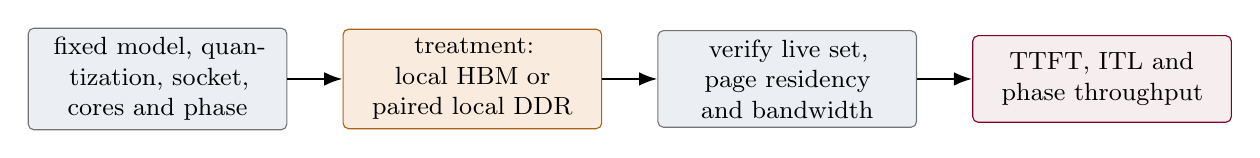
\begin{tikzpicture}[
  >=Latex,
  box/.style={draw=black!55, fill=neutralcol, rounded corners=2pt,
              text width=3.05cm, minimum height=1.1cm,
              align=center, font=\small},
  treatment/.style={box, fill=hbmcol!15, draw=hbmcol!80!black},
  result/.style={box, fill=accent!7, draw=accent}
]
  \node[box] (phase) {fixed model, quantization, socket, cores and phase};
  \node[treatment, right=7mm of phase] (place) {treatment:\\local HBM or paired local DDR};
  \node[box, right=7mm of place] (check) {verify live set, page residency and bandwidth};
  \node[result, right=7mm of check] (out) {TTFT, ITL and phase throughput};
  \draw[->, thick] (phase) -- (place);
  \draw[->, thick] (place) -- (check);
  \draw[->, thick] (check) -- (out);
\end{tikzpicture}
\end{center}

\begin{table}[h]
\centering
\small
\begin{tabularx}{\textwidth}{@{}P{3.4cm}Y@{}}
\toprule
\textbf{Element} & \textbf{Initial design} \\
\midrule
Treatments
& Flat-mode whole-process binding to one socket's local HBM or paired
  local DDR; same pinned binary and workload. \\
Workload points
& At least two model/quantization points that fit comfortably in usable
  local HBM; a small batch/concurrency sweep; fixed prompts and
  generation lengths. \\
Primary outcomes
& Time to first token (TTFT), inter-token latency (ITL), prefill
  throughput and sustained decode throughput. \\
Mechanism checks
& Peak resident live set, pages per NUMA node, achieved tier bandwidth,
  remote traffic, CPU frequency and active AMX/kernel path. \\
Design
& Block by node/allocation; interleave or randomise HBM/DDR order;
  choose repetitions from pilot variance and report effect intervals. \\
\bottomrule
\end{tabularx}
\end{table}

\heading{Decision gates}

\begin{enumerate}
  \item \textbf{Qualify the platform.}  Confirm supported memory mode,
        usable tier capacity, NUMA pairing and a repeatable local/remote
        bandwidth distinction.
  \item \textbf{Answer \researchq{1}.}  Complete the phase-resolved HBM/DDR
        comparison without modifying the runtime.
  \item \textbf{Map the capacity boundary.}  Vary model/quantization,
        context and concurrency; account for weights, packed copies, KV
        and scratch space.
  \item \textbf{Test topology if controls exist.}  Compare one socket,
        two socket-local replicas and a spanning negative control.
  \item \textbf{Modify software only if justified.}  Selective
        weight/KV placement starts only if HBM helps, capacity limits
        the live set, and existing controls cannot express the desired
        split.
\end{enumerate}

\heading{Core thesis completion point}

Platform qualification, \researchq{1}, and a defensible capacity boundary form
a complete empirical thesis.  Topology strengthens the result.
Selective tiering is an optional systems contribution, not a dependency
for thesis completion.

\newpage

{\Large\bfseries\color{accent} Decisions requested from the supervisors\par}
\vspace{3pt}\hrule height 0.35pt\vspace{5pt}

\heading{Questions for the meeting}

\begin{enumerate}
  \item Is the primary contribution appropriately scoped as a
        same-socket, phase-resolved HBM/DDR study?
  \item Which model families and quantizations are scientifically useful
        and operationally available on CRESCO8?
  \item Can the project obtain exclusive Max~9480 nodes, Flat mode,
        reliable NUMA residency data and memory-bandwidth/UPI counters?
  \item Should the core thesis include the capacity/KV boundary, with
        topology treated as secondary?
  \item What standard is expected before calling the gap novel beyond
        the supplied corpus (databases, date range and related runtime
        systems)?
\end{enumerate}

\heading{Main risks and planned response}

\begin{table}[h]
\centering
\footnotesize
\begin{tabularx}{\textwidth}{@{}P{3.0cm}YY@{}}
\toprule
\textbf{Risk} & \textbf{Why it matters} & \textbf{Response} \\
\midrule
File-backed pages or first touch defeat the requested placement
& The treatment label would not correspond to physical memory.
& Inspect pages after loading/warm-up; use an approved cold/warm
  protocol and a non-mmap control when needed. \\
\addlinespace
HBM gain is inferred from STREAM
& Microbenchmark bandwidth is an upper-bound mechanism, not an LLM
  prediction.
& Measure phase bandwidth and explain effect size relative to, not from,
  the local STREAM ratio. \\
\addlinespace
Runtime implementation is chosen too early
& A large patch introduces new confounders and may solve no measured
  problem.
& Freeze an unmodified baseline; require evidence and an ablation before
  selective-tier work. \\
\addlinespace
Capacity is inferred from model-file size
& Packed weights, KV and scratch allocations can cross HBM earlier.
& Record peak live set and pages by tier; retain allocation failures and
  fallback behaviour. \\
\addlinespace
Claims extend beyond the evidence
& One platform/runtime does not represent every CPU or LLM.
& State conclusions for tested configurations and tie transfer to
  measured intensity, live set and locality. \\
\bottomrule
\end{tabularx}
\end{table}

\heading{Immediate next step}

Obtain one pilot allocation and produce a dated platform manifest,
local-HBM/local-DDR bandwidth measurements, a reproducible pinned
\texttt{llama.cpp} build, and a small-model residency check.  Those
observations will determine the final experiment matrix and expose any
operational blocker before the thesis proposal is frozen.

\vfill
{\footnotesize
\setlength{\bibsep}{1pt}
\renewcommand{\bibsection}{\textbf{\color{accent}Selected references}\par}
\bibliographystyle{unsrtnat}
\bibliography{../../thesis/references}
}

\end{document}
